\begin{figure}[t]
    \centering
    \resizebox{\textwidth}{!}{
    \begin{tikzpicture}

    % ==============================
    % Part A (2 clusters)
    % ==============================
    \node at (0, 2cm) {\textbf{(A) The case with 2 clusters.}};

    \node (ligne_1) at (0, 0) {};

    \node[] at ($(ligne_1) + (-3.5cm, 0cm)$) {
    \begin{minipage}{8.5cm}
        \centering
        \begin{tikzpicture}
            % First image
            \node[anchor=south west,inner sep=0] (image1) at (0,0) {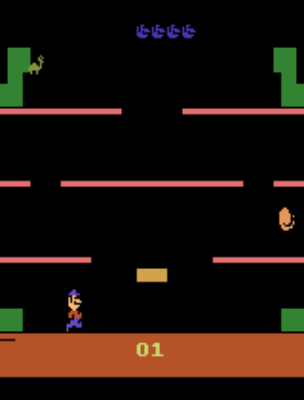
\includegraphics[width=2cm]{figures/clustering_agent_representation/pictures/mario_bros/2_clusters/bloc_pow_available/image_1.png}};
            \begin{scope}[shift={(image1.south west)}, x={(image1.south east)}, y={(image1.north west)}]
                \draw[red, line width=1pt] (0.4,0.275) rectangle (0.6,0.355);
            \end{scope}

            % Second image
            \node[anchor=south west,inner sep=0] (image2) at (image1.south east) [xshift=0.05cm] {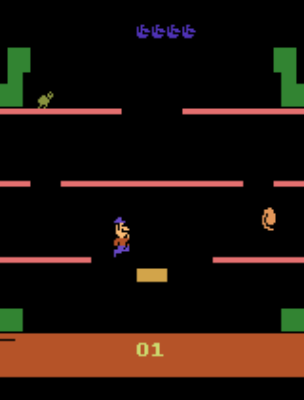
\includegraphics[width=2cm]{figures/clustering_agent_representation/pictures/mario_bros/2_clusters/bloc_pow_available/image_2.png}};
            \begin{scope}[shift={(image2.south west)}, x={(image2.south east)}, y={(image2.north west)}]
                \draw[red, line width=1pt] (0.4,0.275) rectangle (0.6,0.355);
            \end{scope}

            % Third image
            \node[anchor=south west,inner sep=0] (image3) at (image2.south east) [xshift=0.05cm] {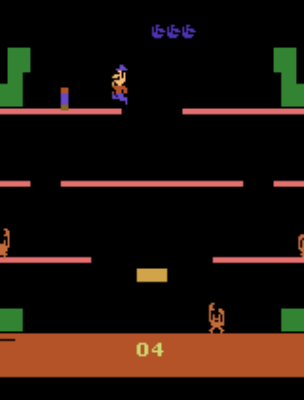
\includegraphics[width=2cm]{figures/clustering_agent_representation/pictures/mario_bros/2_clusters/bloc_pow_available/image_3.png}};
            \begin{scope}[shift={(image3.south west)}, x={(image3.south east)}, y={(image3.north west)}]
                \draw[red, line width=1pt] (0.4,0.275) rectangle (0.6,0.355);
            \end{scope}
        \end{tikzpicture}

        \small The POW block is present.
    \end{minipage}
    };

    \node[] at ($(ligne_1) + (3.5cm, 0cm)$) {
    \begin{minipage}{8.5cm}
        \centering
        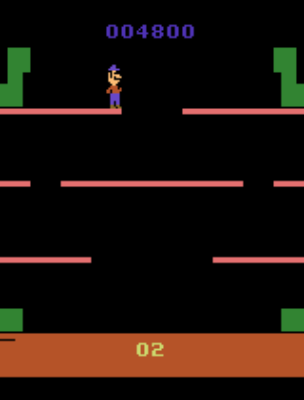
\includegraphics[width=2cm]{figures/clustering_agent_representation/pictures/mario_bros/2_clusters/bloc_pow_available_not/image_1.png}
        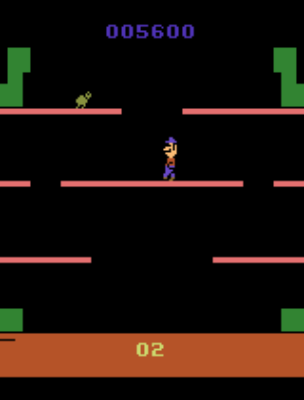
\includegraphics[width=2cm]{figures/clustering_agent_representation/pictures/mario_bros/2_clusters/bloc_pow_available_not/image_2.png}
        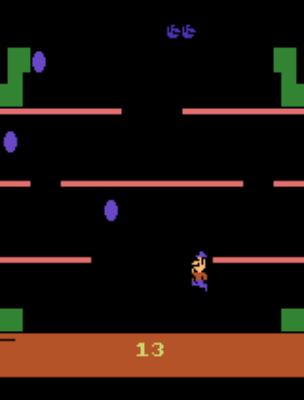
\includegraphics[width=2cm]{figures/clustering_agent_representation/pictures/mario_bros/2_clusters/bloc_pow_available_not/image_3.png}

        \small The POW block is absent.
    \end{minipage}
    };

    % ==============================
    % Separation line
    % ==============================
    \draw[dashed, thick] (-7,-2cm) -- (7,-2cm);

    % ==============================
    % Part B (5 clusters)
    % ==============================
    \node at (0, -2.5cm) {\textbf{(B) The case with 5 clusters.}};

    \node (ligne_2) at (0, -4.5cm) {};

    \node[] at ($(ligne_2) + (-4.5cm, 0cm)$) {
    \begin{minipage}{4.5cm}
        \centering
        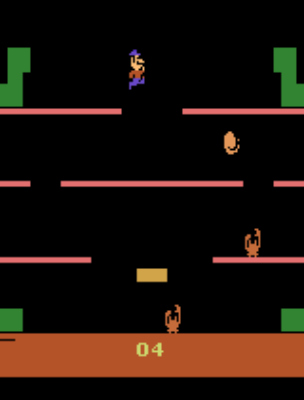
\includegraphics[width=2cm]{figures/clustering_agent_representation/pictures/mario_bros/5_clusters/bloc_pow_available/image_1.png}
        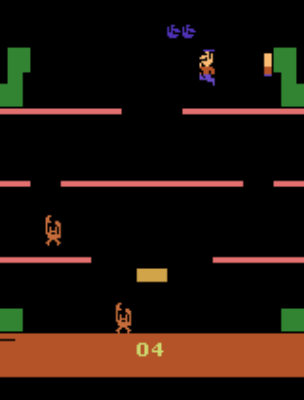
\includegraphics[width=2cm]{figures/clustering_agent_representation/pictures/mario_bros/5_clusters/bloc_pow_available/image_2.png}

        \small The POW block is present.
    \end{minipage}
    };

    \node[] at ($(ligne_2) + (0cm, 0cm)$) {
    \begin{minipage}{4.5cm}
        \centering
        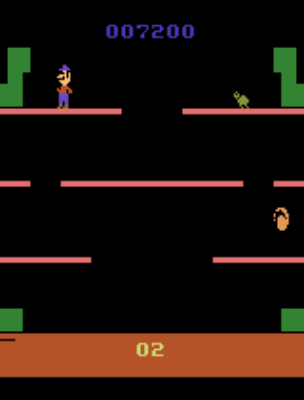
\includegraphics[width=2cm]{figures/clustering_agent_representation/pictures/mario_bros/5_clusters/move_on_top_left_platform/image_1.png}
        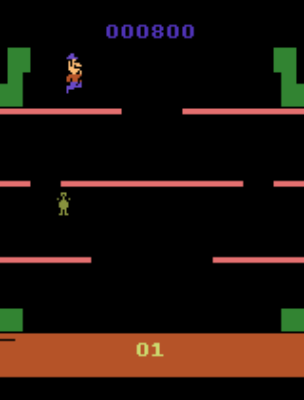
\includegraphics[width=2cm]{figures/clustering_agent_representation/pictures/mario_bros/5_clusters/move_on_top_left_platform/image_3.png}

        \small Move on the left platform.
    \end{minipage}
    };

    \node[] at ($(ligne_2) + (4.5cm, 0cm)$) {
    \begin{minipage}{4.5cm}
        \centering
        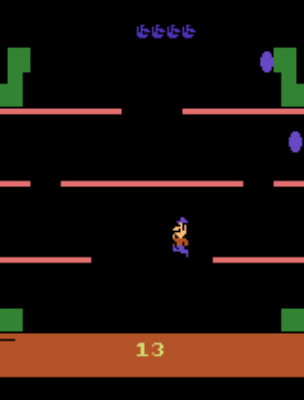
\includegraphics[width=2cm]{figures/clustering_agent_representation/pictures/mario_bros/5_clusters/move_through_level/image_1.png}
        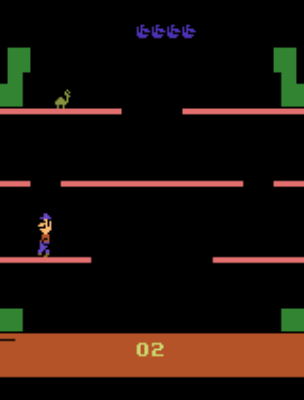
\includegraphics[width=2cm]{figures/clustering_agent_representation/pictures/mario_bros/5_clusters/move_through_level/image_2.png}

        \small Navigating through the level.
    \end{minipage}
    };

    \node[] (g5) at ($(ligne_2) + (-2.25cm, -3.5cm)$) {
    \begin{minipage}{4.5cm}
        \centering
        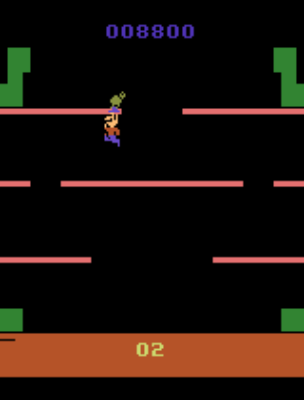
\includegraphics[width=2cm]{figures/clustering_agent_representation/pictures/mario_bros/5_clusters/neutralize_enemies_left/image_1.png}
        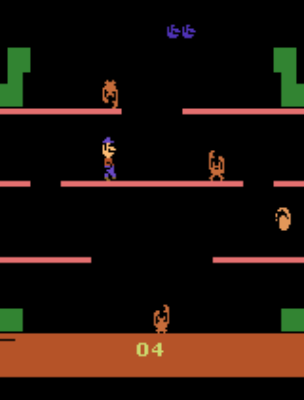
\includegraphics[width=2cm]{figures/clustering_agent_representation/pictures/mario_bros/5_clusters/neutralize_enemies_left/image_3.png}

        \small Attacking the left.
    \end{minipage}
    };

    \node[] at ($(ligne_2) + (2.25cm, -3.5cm)$) {
    \begin{minipage}{4.5cm}
        \centering
        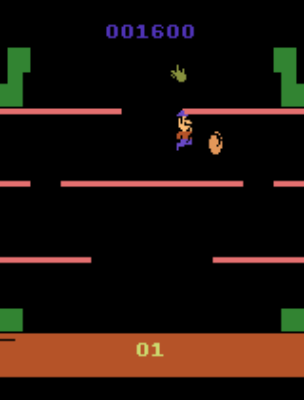
\includegraphics[width=2cm]{figures/clustering_agent_representation/pictures/mario_bros/5_clusters/neutralize_enemies_right/image_1.png}
        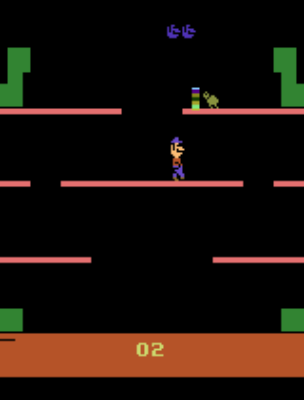
\includegraphics[width=2cm]{figures/clustering_agent_representation/pictures/mario_bros/5_clusters/neutralize_enemies_right/image_2.png}

        \small Attacking the right.
    \end{minipage}
    };

    \end{tikzpicture}
    }
    \caption{Effect of the number of clusters on the groupings identified by \gls{car} in the Mario Bros environment.}
    \label{fig:semantic_granularity}
\end{figure}
